%
% streckenvergleich.tex
%
% (c) 2018 Prof Dr Andreas Müller, Hochschule Rapperswil
%
\documentclass[tikz,12pt]{standalone}
\usepackage{times}
\usepackage{amsmath}
\usepackage{txfonts}
\usepackage[utf8]{inputenc}
\usepackage{graphics}
\usepackage{color}
\usepackage{pifont}
\usetikzlibrary{arrows,intersections,math,calc}
\begin{document}

\def\punkt#1{
        \fill[color=white] #1 circle[radius=0.08];
        \draw #1 circle[radius=0.08];
}

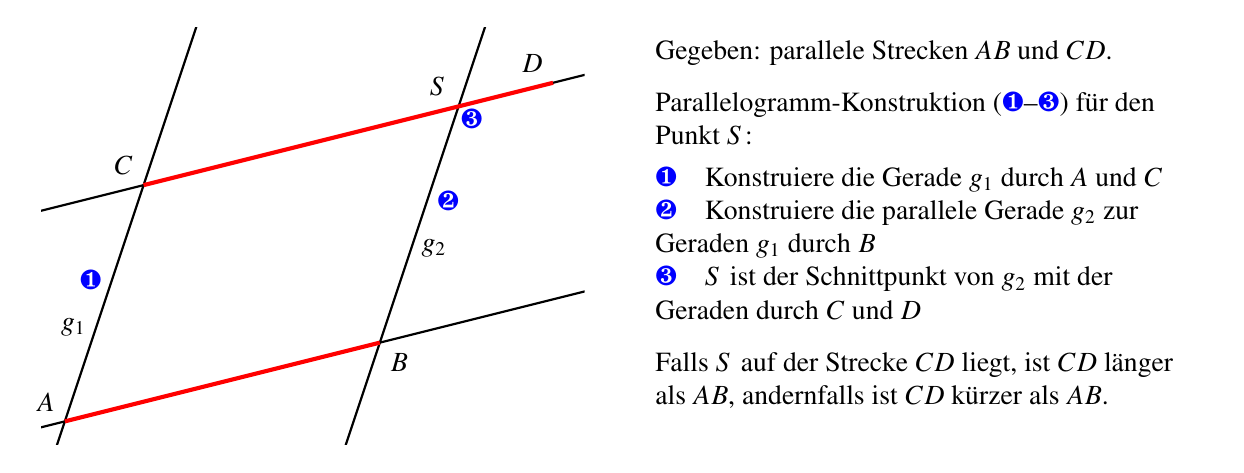
\begin{tikzpicture}[>=latex,thick]

\coordinate (O) at (0,0);
\coordinate (A) at (4,1);
\coordinate (B) at (1,3);
\coordinate (C) at ($(B)+1.3*(A)$);

\begin{scope}
\clip (-0.3,-0.3) rectangle (6.6,5.0);

\draw ($(B)-(A)$)--($(B)+2*(A)$);
\draw ($(O)-(A)$)--($(A)+(A)$);

\draw ($(O)-(B)$)--($2*(B)$);
\draw ($(A)-(B)$)--($(A)+2*(B)$);

\end{scope}

\draw[color=red,line width=1.5pt] (O)--(A);
\draw[color=red,line width=1.5pt] (B)--(C);

\punkt{(O)} \node at (O) [above left] {$A$};
\punkt{(A)} \node at (A) [below right] {$B$};
\punkt{(B)} \node at (B) [above left] {$C$};
\punkt{(C)} \node at (C) [above left] {$D$};

\coordinate (S) at ($(A)+(B)$);

\punkt{(S)} \node at (S) [above left] {$S$};
\node at ($(S)+(-0.1,0.1)$) [below right] {\color{blue}\ding{184}};

\node at ($0.4*(B)$) [left] {$g_1$};
\node at ($0.6*(B)$) [left] {\color{blue}\ding{182}};
\node at ($(A)+0.4*(B)$) [right] {$g_2$};
\node at ($(A)+0.6*(B)$) [right] {\color{blue}\ding{183}};

\node at (11.0,2.5) {%
\begin{minipage}{7.0cm}
\parindent0pt
\raggedright
Gegeben: parallele Strecken $AB$ und $CD$.\\[7pt]
Parallelogramm-Konstruktion ({\color{blue}\ding{182}}--{\color{blue}\ding{184}})
für den Punkt $S$:\\[3pt]
{\color{blue}\ding{182}}\quad%
Konstruiere die Gerade $g_1$ durch $A$ und $C$\\
{\color{blue}\ding{183}}\quad%
Konstruiere die parallele Gerade $g_2$ zur Geraden $g_1$ durch $B$\\
{\color{blue}\ding{184}}\quad%
$S$ ist der Schnittpunkt von $g_2$ mit der Geraden durch $C$ und $D$\\[7pt]
%{\color{blue}\ding{185}}\quad%
Falls $S$ auf der Strecke $CD$ liegt, ist $CD$ länger als $AB$,
andernfalls ist $CD$ kürzer als $AB$.
\end{minipage}};

\end{tikzpicture}

\end{document}

